\documentclass[11pt,a4paper]{uebung}

\usepackage[british]{babel}
\usepackage{epsfig}
\usepackage{rotate}
\usepackage{amsmath,amsthm,amssymb}
\usepackage{color}
\makeatletter\let\@amsfonts=P\makeatother
\usepackage{graphicx}
\usepackage{typearea}
\usepackage{multicol}
\usepackage{amsfonts}
\usepackage[nounderscore]{syntax}
\usepackage{enumitem}
\newcommand{\comment}[1]{\marginpar{\small{\bf Comment:} #1}}

\usepackage{tikz}
\usetikzlibrary{shapes,arrows,backgrounds,%
matrix,patterns,arrows,decorations.pathmorphing,decorations.pathreplacing,%
positioning,fit,calc,decorations.text,shadows%
}

\newcommand{\solution}[1]{\par {\bf Solution:}\\#1}



%put your Matrikelnummer here instead of the XXXXXXXX
% if your group has less than 3 members, just delete the remaining XXXXXXXX
\newcommand\matrikelnummerA[0]{XXXXXXXX}
\newcommand\matrikelnummerB[0]{XXXXXXXX}
\newcommand\matrikelnummerC[0]{0608292}
%put your Matrikelnummer here instead of the XXXXXXXX



\def\cT{\mathcal{T}}


\begin{document}
\newcommand{\Vorlesung}{Formal Methods in Computer Science}
\newcommand{\Semester}{SS 2012}
\newcommand{\Prof}{Uwe Egly}
\newcommand{\AssisA}{Antonius Weinzierl}
\newcommand{\AssisB}{}

%%%%%%%%%%%%%%%%%%%%%%%%%%%%%%%%%%%%%%%%%%%%%%%%%%%%%%%%%%%%%%%%%%%%%%%%%%%%%%

\Uebungsblatt{2 (10 points)}{
  \begin{tabular}{rl}
   Matrikelnummer(n): &\matrikelnummerA \\
   &\matrikelnummerB \\
   &\matrikelnummerC
  \end{tabular}
}

%%%%%%%%%%%%%%%%%%%%%%%%%%%%%%%%%%%%%%%%%%%%%%%%%%%%%%%%%%%%%%%%%%%%%%%%%%%%%%


\Aufgabe[Tseitin Transformation \hfill \bf (0.5 + 1 + 1.5 points)]

\begin{enumerate}
\item Extend Tseitin's transformation for the connectives $\leftrightarrow$
  (equivalence) and $\oplus$ (XOR). Find the necessary clauses for the new schemes
  $l_i \leftrightarrow (l_{i'} \leftrightarrow l_{i''})$ and $l_k
  \leftrightarrow (l_{k'} \oplus l_{k''})$.
  
  \solution{
Construct the equivalences for the SFOs and translate the labeled
subformulas to CNF (local constraints):

% use packages: array
\begin{tabular}{|l|l|l|l|}
\hline
\textsl{\small Equivalences} & \multicolumn{3}{c|}{\textsl{\small Associated
Clauses}} \\ 
{\small \textsl{for SFOs in} $\phi $} & $C_{1}(\phi )$ & $C_{2}(\phi )$ & $%
C_{3}(\phi )$ \\ \hline
$I_{1}\IFF x$ & $\lnot I_{1}\OR x$ & $I_{1}\OR\lnot x$ &  \\ 
$I_{2}\IFF y$ & $\lnot I_{2}\OR y$ & $I_{2}\OR\lnot y$ &  \\ 
$I_{3}\IFF(I_{1}\AND I_{2})$ & $\lnot I_{3}\OR I_{1}$ & $\lnot I_{3}\OR %
I_{2} $ & $I_{3}\OR\lnot I_{1}\OR\lnot I_{2}$ \\ 
$I_{4}\IFF y$ & $\lnot I_{4}\OR y$ & $I_{4}\OR\lnot y$ &  \\ 
$I_{5}\IFF z$ & $\lnot I_{5}\OR z$ & $I_{5}\OR\lnot z$ &  \\ 
$I_{6}\IFF(I_{4}\AND I_{5})$ & $\lnot I_{6}\OR I_{4}$ & $\lnot I_{6}\OR %
I_{5} $ & $I_{6}\OR\lnot I_{4}\OR\lnot I_{5}$ \\ 
$I_{7}\IFF z$ & $\lnot I_{7}\OR z$ & $I_{7}\OR\lnot z$ &  \\ 
$I_{8}\IFF\lnot I_{7}$ & $\lnot I_{8}\OR\lnot I_{7}$ & $I_{8}\OR I_{7}$ & 
\\ 
$I_{9}\IFF(I_{3}\IMPL I_{6})$ & $\lnot I_{9}\OR\lnot I_{3}\OR I_{6}$ & $I_{9}%
\OR I_{3}$ & $I_{9}\OR\lnot I_{6}$ \\ 
$I_{10}\IFF(I_{9}\IMPL I_{8})$ & $\lnot I_{10}\OR\lnot I_{9}\OR I_{8}$ & $%
I_{10}\OR I_{9}$ & $I_{10}\OR\lnot I_{8}$ \\ \hline
\end{tabular}
\label{tab:translation_cnf}

  }

\item Apply Tseitin's transformation to the following formula $\psi$: $a \rightarrow
  \big( b \lor \neg (a \leftrightarrow c)\big)$.
  
  Hint: You do not need to introduce labels for propositions $a,b,$ and $c$.
  \solution{
  }

\item Let $\psi$ be a propositional formula and $D^\psi$ the set of clauses
  resulting from Tseitin's transformation on $\psi$. Prove that the following
  holds:
  
  \centerline{If $\psi$ is satisfiable then $D^\psi$ is satisfiable.}

  You only need to prove this for the connectives $\land$ and $\neg$.
  %\lor,\neg, \rightarrow$.
  Use the below clause schemes, which introduce a new label for every boolean
  variable.
  \begin{align*}
    L_a \leftrightarrow a && (\neg L_a \lor a)&& (L_a \lor \neg a)\\
    L_\phi \leftrightarrow (L_1 \land L_2) && (\neg L_\phi \lor L_1)&& (\neg
    L_\phi \lor L_2)&& (L_\phi \lor \neg L_1 \lor \neg L_2)\\
    L_\phi \leftrightarrow \neg L_1 && (\neg L_\phi \lor \neg L_1)&& (L_\phi
    \lor L_1)
  \end{align*}
  
  \solution{
  }
\end{enumerate}


%%%%%%%%%%%%%%%%%%%%%%%%%%%%%%%%%%%%%%%%%%%%%%%%%%%%%%%%%%%%%%%%%%%%%%%%%%%%%%

\newpage
\Aufgabe[Implication Graphs \hfill \bf (2+1+1.5 points)]
\begin{enumerate}
\item Let $\mathcal{D}$ be the following set of clauses:
  \begin{align*}
    c_1:& (A \lor B)\\
    c_2:& (A \lor G \lor H)\\
    c_3:& (\neg B \lor \neg D \lor E)\\
    c_4:& (E \lor F)\\
    c_5:& (\neg F \lor \neg G \lor D)\\
    c_6:& (\neg C \lor G \lor J)\\
    c_7:& (\neg J \lor \neg H)
  \end{align*}
  Draw the implication graph resulting from $\mathcal{D}$ with decisions
  $A=0@1$, $C=1@2$, $E=0@3$. Find the first UIP, and learn a new clause using
  the first-UIP scheme (use resolution).

  \solution{
Implication graph:\medskip

%TCIMACRO{%
%\TeXButton{Decision tree}{\begin{tikzpicture}[node distance=2.5cm,auto]
%\node (D) {D=0@2};
%\node (B) [above right of=D] {B=1@2};
%\node (C) [below right of=D] {C=0@2};
%\node (A) [right of=B] {A=0@1};
%\node (K) [right of=C] {$\mathcal K$};
%\path[->] (D) edge node {$C_2$} (B);
%\path[->] (D) edge node {$C_3$} (C);
%\path[->] (B) edge node {$C_1$} (K);
%\path[->] (C) edge node {$C_1$} (K);
%\path[->] (A) edge node {$C_1$} (K);
%\end{tikzpicture}}}%
%BeginExpansion
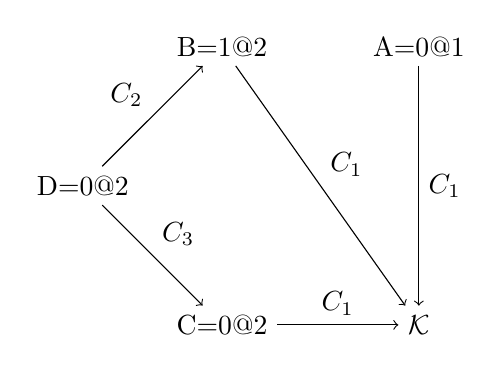
\begin{tikzpicture}[node distance=2.5cm,auto]
\node (D) {D=0@2};
\node (B) [above right of=D] {B=1@2};
\node (C) [below right of=D] {C=0@2};
\node (A) [right of=B] {A=0@1};
\node (K) [right of=C] {$\mathcal K$};
\path[->] (D) edge node {$C_2$} (B);
\path[->] (D) edge node {$C_3$} (C);
\path[->] (B) edge node {$C_1$} (K);
\path[->] (C) edge node {$C_1$} (K);
\path[->] (A) edge node {$C_1$} (K);
\end{tikzpicture}%
%EndExpansion
\newline
\bigskip

  }

\item Prove that in a conflict graph the first UIP is uniquely defined, i.e.,
  prove that there is exactly one node in the graph which is a first UIP.

  \solution{
  }

\item Let $\mathcal{C}$ be a set of clauses and $G$ a conflict graph with
  respect to $\mathcal{C}$. Prove: if a clause $C_l$ is learned following the
  first-UIP scheme, then $C_l$ is a consequence of $\mathcal{C}$.

  \solution{
  }
\end{enumerate}


%%%%%%%%%%%%%%%%%%%%%%%%%%%%%%%%%%%%%%%%%%%%%%%%%%%%%%%%%%%%%%%%%%%%%%%%%%%%%%

\newpage
\Aufgabe[Sparse Method \hfill \bf (1.5 points)]
Apply the Sparse Method including preprocessing on the formula $\varphi^E$
below to obtain a propositional formula.
\begin{displaymath}
  (x_1 \neq x_2 \lor x_2=x_3 ) \land \big[ (x_2 \neq x_4 \land x_3=x_4
  \land x_4=x_5)
  \lor (x_6 \neq x_5 \land x_6=x_7 \land x_7=x_3)\big]
\end{displaymath}

  \solution{
The sparse method is a decision procedure for equality logic that computes
equi-satisfiable formulas in propositional logic.

Consider formula $\varphi ^{E}$ in equation logic:%

\begin{displaymath}
  \varphi ^{E}: (x_1 \neq x_2 \lor x_2=x_3 ) \land \big[ (x_2 \neq x_4 \land x_3=x_4
  \land x_4=x_5)
  \lor (x_6 \neq x_5 \land x_6=x_7 \land x_7=x_3)\big]
\end{displaymath}

Then the sets of equality literals and disequality literals of $\varphi ^{E}$
are:

\begin{eqnarray*}
E_{=}
&=&%
\{x_{2}=x_{3,}x_{3}=x_{4},x_{4}=x_{5},x_{6}=x_{7},x_{7}=x_{3}\}
\\
E_{\neq } &=&\{x_{1}\neq x_{2},x_{2}\neq x_{4},x_{6}\neq x_{5}\}
\end{eqnarray*}

It is very often the case, that a given equality logic formula $\varphi ^{E}$
can be simplified. Before reducing $\varphi ^{E}$ to a propositional formula 
$\varphi ^{P}$, we have to do some preprocessing for simplifying the
equality formula $\varphi ^{E}$:

\begin{enumerate}
\item Construct an equality graph $G^{E}(\varphi ^{E})=(V,E_{=},E_{\neq })$:

%TCIMACRO{%
%\TeXButton{Equality graph}{\begin{tikzpicture}[>=latex',line join=bevel,]
%\pgfsetlinewidth{1bp}
%\pgfsetcolor{black}
% \draw [solid] (229.02bp,163.94bp) .. controls (246.01bp,158.42bp) and (274.84bp,149.06bp)  .. (291.75bp,143.56bp);
% \draw [dotted] (305.23bp,124.42bp) .. controls (305.23bp,106.67bp) and (305.23bp,77.061bp)  .. (305.23bp,59.357bp);
%\definecolor{strokecol}{rgb}{0.0,0.0,0.0};
%\pgfsetstrokecolor{strokecol}
%\draw (300.23bp,91.888bp) node {$=$};
% \draw [solid] (102.06bp,91.939bp) .. controls (114.68bp,91.939bp) and (133.03bp,91.939bp)  .. (145.64bp,91.939bp);
% \draw [dotted] (15.5bp,64.726bp) .. controls (15.5bp,79.963bp) and (15.5bp,103.76bp)  .. (15.5bp,119.04bp);
%\draw (10.5bp,91.883bp) node {$=$};
% \draw [dotted] (27.771bp,57.261bp) .. controls (40.992bp,64.894bp) and (61.924bp,76.979bp)  .. (75.262bp,84.68bp);
%\draw (56.516bp,62.97bp) node {$=$};
% \draw [dotted] (168.27bp,80.33bp) .. controls (178.71bp,65.963bp) and (196.38bp,41.636bp)  .. (206.86bp,27.219bp);
%\draw (180.56bp,48.774bp) node {$=$};
% \draw [dotted] (27.771bp,126.62bp) .. controls (40.992bp,118.98bp) and (61.924bp,106.9bp)  .. (75.262bp,99.199bp);
%\draw (56.516bp,120.91bp) node {$=$};
% \draw [solid] (296.62bp,127.32bp) .. controls (279.4bp,103.62bp) and (240.92bp,50.664bp)  .. (223.83bp,27.143bp);
% \draw [dotted] (168.27bp,103.55bp) .. controls (178.71bp,117.92bp) and (196.38bp,142.24bp)  .. (206.86bp,156.66bp);
%\draw (194.56bp,125.1bp) node {$=$};
% \draw [dotted] (229.02bp,19.934bp) .. controls (246.01bp,25.454bp) and (274.84bp,34.822bp)  .. (291.75bp,40.317bp);
%\draw (263.39bp,21.126bp) node {$=$};
%\begin{scope}
%\definecolor{strokecol}{rgb}{0.0,0.0,0.0};
%\pgfsetstrokecolor{strokecol}
%\draw (305bp,45bp) ellipse (14bp and 15bp);
%\draw (305.23bp,44.697bp) node {$x_6$};
%\end{scope}
%\begin{scope}
%\definecolor{strokecol}{rgb}{0.0,0.0,0.0};
%\pgfsetstrokecolor{strokecol}
%\draw (305bp,139bp) ellipse (14bp and 15bp);
%\draw (305.23bp,139.18bp) node {$x_7$};
%\end{scope}
%\begin{scope}
%\definecolor{strokecol}{rgb}{0.0,0.0,0.0};
%\pgfsetstrokecolor{strokecol}
%\draw (215bp,15bp) ellipse (14bp and 15bp);
%\draw (215.37bp,15.5bp) node {$x_5$};
%\end{scope}
%\begin{scope}
%\definecolor{strokecol}{rgb}{0.0,0.0,0.0};
%\pgfsetstrokecolor{strokecol}
%\draw (160bp,92bp) ellipse (14bp and 15bp);
%\draw (159.84bp,91.939bp) node {$x_4$};
%\end{scope}
%\begin{scope}
%\definecolor{strokecol}{rgb}{0.0,0.0,0.0};
%\pgfsetstrokecolor{strokecol}
%\draw (215bp,168bp) ellipse (14bp and 15bp);
%\draw (215.37bp,168.38bp) node {$x_3$};
%\end{scope}
%\end{tikzpicture}
%}}%
%BeginExpansion
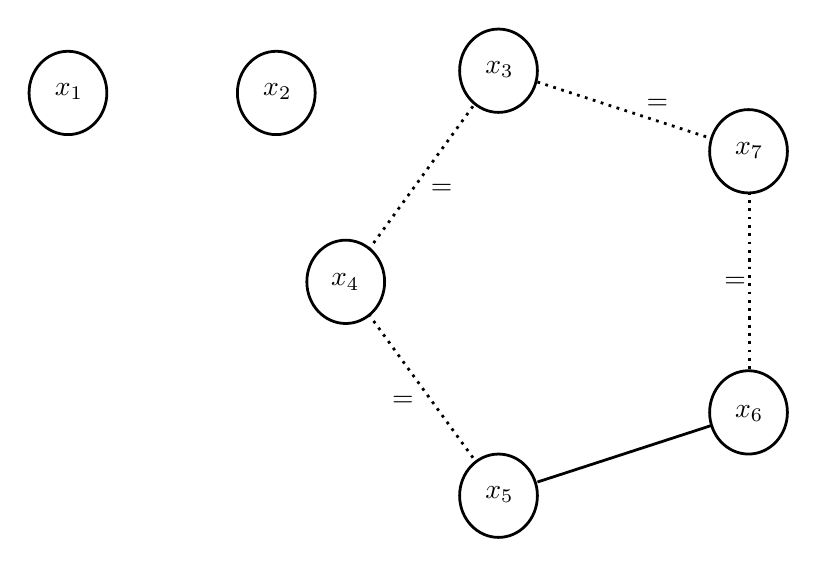
\begin{tikzpicture}[>=latex',line join=bevel,]
\pgfsetlinewidth{1bp}
\pgfsetcolor{black}
\draw (272.23bp,155.888bp) node {$=$};
 \draw [dotted] (229.02bp,163.94bp) .. controls (246.01bp,158.42bp) and (274.84bp,149.06bp)  .. (291.75bp,143.56bp);
 \draw [dotted] (305.23bp,124.42bp) .. controls (305.23bp,106.67bp) and (305.23bp,77.061bp)  .. (305.23bp,59.357bp);
\definecolor{strokecol}{rgb}{0.0,0.0,0.0};
\pgfsetstrokecolor{strokecol}
\draw (300.23bp,91.888bp) node {$=$};
 \draw [dotted] (168.27bp,80.33bp) .. controls (178.71bp,65.963bp) and (196.38bp,41.636bp)  .. (206.86bp,27.219bp);
\draw (180.56bp,48.774bp) node {$=$};
 \draw [dotted] (168.27bp,103.55bp) .. controls (178.71bp,117.92bp) and (196.38bp,142.24bp)  .. (206.86bp,156.66bp);
\draw (194.56bp,125.1bp) node {$=$};
 \draw [solid] (229.02bp,19.934bp) .. controls (246.01bp,25.454bp) and (274.84bp,34.822bp)  .. (291.75bp,40.317bp);
\begin{scope}
\definecolor{strokecol}{rgb}{0.0,0.0,0.0};
\pgfsetstrokecolor{strokecol}
\draw (305bp,45bp) ellipse (14bp and 15bp);
\draw (305.23bp,44.697bp) node {$x_6$};
\end{scope}
\begin{scope}
\definecolor{strokecol}{rgb}{0.0,0.0,0.0};
\pgfsetstrokecolor{strokecol}
\draw (305bp,139bp) ellipse (14bp and 15bp);
\draw (305.23bp,139.18bp) node {$x_7$};
\end{scope}
\begin{scope}
\definecolor{strokecol}{rgb}{0.0,0.0,0.0};
\pgfsetstrokecolor{strokecol}
\draw (215bp,15bp) ellipse (14bp and 15bp);
\draw (215.37bp,15.5bp) node {$x_5$};
\end{scope}
\begin{scope}
\definecolor{strokecol}{rgb}{0.0,0.0,0.0};
\pgfsetstrokecolor{strokecol}
\draw (160bp,92bp) ellipse (14bp and 15bp);
\draw (159.84bp,91.939bp) node {$x_4$};
\end{scope}
\begin{scope}
\definecolor{strokecol}{rgb}{0.0,0.0,0.0};
\pgfsetstrokecolor{strokecol}
\draw (215bp,168bp) ellipse (14bp and 15bp);
\draw (215.37bp,168.38bp) node {$x_3$};
\end{scope}
\begin{scope}
\definecolor{strokecol}{rgb}{0.0,0.0,0.0};
\pgfsetstrokecolor{strokecol}
\draw (135bp,160bp) ellipse (14bp and 15bp);
\draw (135.37bp,160.38bp) node {$x_2$};
\end{scope}
\begin{scope}
\definecolor{strokecol}{rgb}{0.0,0.0,0.0};
\pgfsetstrokecolor{strokecol}
\draw (60bp,160bp) ellipse (14bp and 15bp);
\draw (60.37bp,160.38bp) node {$x_1$};
\end{scope}
\end{tikzpicture}
%
%EndExpansion

The equality graph has two contradictory cycles, $%
c_{1}=(x_{6},x_{8},x_{7},x_{6})$ and $%
c_{2}=(x_{4},x_{5},x_{6},x_{8},x_{7},x_{4})$.

\item Simplifying the graph $G^{E}(\varphi ^{E})$ by replacing each pure
literal in $\varphi ^{E}$ whose corresponding edge is not part of a simple
contradictory cycle with \textsc{True}.

According to the algorithm, $G^{E}(\varphi _{1}^{E})$ can be further
simplified by replacing literals with \textsc{True}:
\bigskip
\end{enumerate}

Following strictly the rules of the simplification algorithm, the algorithm
replace in this case every literal in the equality formula $\varphi ^{E}$
with \textsc{True}. In order to transform $\varphi ^{E}$ into a
propositional formula $\varphi ^{P}$, we have to make a little trick to
enforce the application of the reduction algorithm. In this case we apply
only one step of the simplification algorithm and replace all literals at
once with \textsc{True}, which are not in the cycles $c_{1}$ and $c_{2}$. So
we get:

\begin{eqnarray*}
\varphi _{1}^{E} &:&(\text{\textsc{True}}\vee \text{\textsc{True}})\wedge (%
\text{\textsc{True}})\wedge (x_{3}\,{\neq }\,x_{4}\vee x_{5}\,{\neq }%
\,x_{6})\wedge \\
(x_{4}\, &{=}&\,x_{5}\vee x_{4}\,{=}\,x_{7}\vee x_{6}\,{\neq }\,x_{7})\wedge
(x_{6}\,{=}\,x_{8}\vee x_{7}\,{=}\,x_{8})
\end{eqnarray*}

\begin{equation*}
\Rightarrow \;\;\varphi _{1}^{E}:(x_{3}\,{\neq }\,x_{4}\vee x_{5}\,{\neq }%
\,x_{6})\wedge (x_{4}\,{=}\,x_{5}\vee x_{4}\,{=}\,x_{7}\vee x_{6}\,{\neq }%
\,x_{7})\wedge (x_{6}\,{=}\,x_{8}\vee x_{7}\,{=}\,x_{8})
\end{equation*}

Then the equality graph $G^{E}(\varphi _{1}^{E})$ looks like:

%TCIMACRO{%
%\TeXButton{Equality graph 1 (variant)}{\begin{tikzpicture}[>=latex',line join=bevel,]
%\pgfsetlinewidth{1bp}
%\pgfsetcolor{black}
% \draw [solid] (15.5bp,59.46bp) .. controls (15.5bp,77.211bp) and (15.5bp,106.82bp)  .. (15.5bp,124.52bp);
% \draw [dotted] (29.148bp,143.62bp) .. controls (46.136bp,149.14bp) and (74.968bp,158.5bp)  .. (91.878bp,164bp);
%\definecolor{strokecol}{rgb}{0.0,0.0,0.0};
%\pgfsetstrokecolor{strokecol}
%\draw (63.513bp,144.81bp) node {$=$};
% \draw [dotted] (152.46bp,103.55bp) .. controls (142.02bp,117.92bp) and (124.35bp,142.24bp)  .. (113.87bp,156.66bp);
%\draw (126.17bp,125.1bp) node {$=$};
% \draw [solid] (28.918bp,134.82bp) .. controls (56.617bp,125.82bp) and (119.84bp,105.28bp)  .. (147.51bp,96.289bp);
% \draw [dotted] (113.79bp,27.11bp) .. controls (124.23bp,41.477bp) and (141.91bp,65.803bp)  .. (152.38bp,80.221bp);
%\draw (140.09bp,48.665bp) node {$=$};
% \draw [dotted] (91.712bp,19.934bp) .. controls (74.724bp,25.454bp) and (45.892bp,34.822bp)  .. (28.982bp,40.317bp);
%\draw (63.347bp,39.126bp) node {$=$};
%\begin{scope}
%\definecolor{strokecol}{rgb}{0.0,0.0,0.0};
%\pgfsetstrokecolor{strokecol}
%\draw (105bp,168bp) ellipse (14bp and 15bp);
%\draw (105.36bp,168.38bp) node {$x_8$};
%\end{scope}
%\begin{scope}
%\definecolor{strokecol}{rgb}{0.0,0.0,0.0};
%\pgfsetstrokecolor{strokecol}
%\draw (16bp,139bp) ellipse (14bp and 15bp);
%\draw (15.5bp,139.18bp) node {$x_6$};
%\end{scope}
%\begin{scope}
%\definecolor{strokecol}{rgb}{0.0,0.0,0.0};
%\pgfsetstrokecolor{strokecol}
%\draw (161bp,92bp) ellipse (14bp and 15bp);
%\draw (160.9bp,91.939bp) node {$x_7$};
%\end{scope}
%\begin{scope}
%\definecolor{strokecol}{rgb}{0.0,0.0,0.0};
%\pgfsetstrokecolor{strokecol}
%\draw (105bp,15bp) ellipse (14bp and 15bp);
%\draw (105.36bp,15.5bp) node {$x_4$};
%\end{scope}
%\begin{scope}
%\definecolor{strokecol}{rgb}{0.0,0.0,0.0};
%\pgfsetstrokecolor{strokecol}
%\draw (15bp,45bp) ellipse (14bp and 15bp);
%\draw (15.5bp,44.697bp) node {$x_5$};
%\end{scope}
%\end{tikzpicture}
%}}%
%BeginExpansion
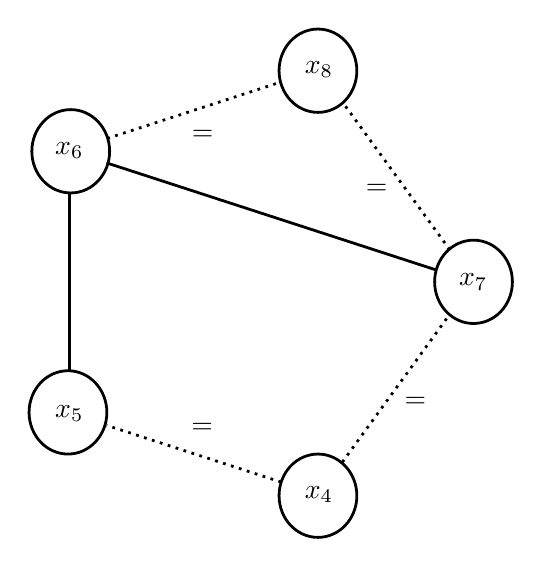
\begin{tikzpicture}[>=latex',line join=bevel,]
\pgfsetlinewidth{1bp}
\pgfsetcolor{black}
 \draw [solid] (15.5bp,59.46bp) .. controls (15.5bp,77.211bp) and (15.5bp,106.82bp)  .. (15.5bp,124.52bp);
 \draw [dotted] (29.148bp,143.62bp) .. controls (46.136bp,149.14bp) and (74.968bp,158.5bp)  .. (91.878bp,164bp);
\definecolor{strokecol}{rgb}{0.0,0.0,0.0};
\pgfsetstrokecolor{strokecol}
\draw (63.513bp,144.81bp) node {$=$};
 \draw [dotted] (152.46bp,103.55bp) .. controls (142.02bp,117.92bp) and (124.35bp,142.24bp)  .. (113.87bp,156.66bp);
\draw (126.17bp,125.1bp) node {$=$};
 \draw [solid] (28.918bp,134.82bp) .. controls (56.617bp,125.82bp) and (119.84bp,105.28bp)  .. (147.51bp,96.289bp);
 \draw [dotted] (113.79bp,27.11bp) .. controls (124.23bp,41.477bp) and (141.91bp,65.803bp)  .. (152.38bp,80.221bp);
\draw (140.09bp,48.665bp) node {$=$};
 \draw [dotted] (91.712bp,19.934bp) .. controls (74.724bp,25.454bp) and (45.892bp,34.822bp)  .. (28.982bp,40.317bp);
\draw (63.347bp,39.126bp) node {$=$};
\begin{scope}
\definecolor{strokecol}{rgb}{0.0,0.0,0.0};
\pgfsetstrokecolor{strokecol}
\draw (105bp,168bp) ellipse (14bp and 15bp);
\draw (105.36bp,168.38bp) node {$x_8$};
\end{scope}
\begin{scope}
\definecolor{strokecol}{rgb}{0.0,0.0,0.0};
\pgfsetstrokecolor{strokecol}
\draw (16bp,139bp) ellipse (14bp and 15bp);
\draw (15.5bp,139.18bp) node {$x_6$};
\end{scope}
\begin{scope}
\definecolor{strokecol}{rgb}{0.0,0.0,0.0};
\pgfsetstrokecolor{strokecol}
\draw (161bp,92bp) ellipse (14bp and 15bp);
\draw (160.9bp,91.939bp) node {$x_7$};
\end{scope}
\begin{scope}
\definecolor{strokecol}{rgb}{0.0,0.0,0.0};
\pgfsetstrokecolor{strokecol}
\draw (105bp,15bp) ellipse (14bp and 15bp);
\draw (105.36bp,15.5bp) node {$x_4$};
\end{scope}
\begin{scope}
\definecolor{strokecol}{rgb}{0.0,0.0,0.0};
\pgfsetstrokecolor{strokecol}
\draw (15bp,45bp) ellipse (14bp and 15bp);
\draw (15.5bp,44.697bp) node {$x_5$};
\end{scope}
\end{tikzpicture}
%
%EndExpansion

Recall the theorem,%
\begin{equation*}
\varphi ^{E}\text{ is satisfiable }\Leftrightarrow e(\varphi ^{E})\AND B_{t}%
\text{ is satisfiable,}
\end{equation*}

where $e(\varphi ^{E})$ denotes the \textit{propositional skeleton} of $%
\varphi ^{E}$and $B_{t}$ is a formula that describes the \textit{%
transitivity constraints} (conjunctions of implications).

So $\varphi ^{P}=e(\varphi ^{E})\AND B_{t}$ is equi-satisfiable to $\varphi
^{E}$, iff $\varphi ^{E}$ is satisfiable.

\begin{enumerate}
\item First we construct the propositional skeleton of $\varphi _{1}^{E}$ by
replacing each atom of the form $x_{i}=x_{j}$ in $\varphi _{1}^{E}$ with $%
e_{i,j}$, such that:%
\begin{equation*}
e(\varphi _{1}^{E})=(e_{4,5}\OR e_{4,7}\OR\lnot e_{6,7})\AND(e_{6,8}\OR %
e_{7,8})\AND(\lnot e_{3,4}\OR\lnot e_{5,6})
\end{equation*}

\item Construct the nonpolar equality graph $G_{NP}^{E}(\varphi _{1}^{E})$:

%TCIMACRO{%
%\TeXButton{Nonpolar equality graph}{\begin{tikzpicture}[>=latex',line join=bevel,]
%\pgfsetlinewidth{1bp}
%\pgfsetcolor{black}
% \draw [solid] (15.5bp,59.46bp) .. controls (15.5bp,77.211bp) and (15.5bp,106.82bp)  .. (15.5bp,124.52bp);
% \draw [solid] (29.148bp,143.62bp) .. controls (46.136bp,149.14bp) and (74.968bp,158.5bp)  .. (91.878bp,164bp);
% \draw [solid] (152.46bp,103.55bp) .. controls (142.02bp,117.92bp) and (124.35bp,142.24bp)  .. (113.87bp,156.66bp);
% \draw [solid] (28.918bp,134.82bp) .. controls (56.617bp,125.82bp) and (119.84bp,105.28bp)  .. (147.51bp,96.289bp);
% \draw [solid] (113.79bp,27.11bp) .. controls (124.23bp,41.477bp) and (141.91bp,65.803bp)  .. (152.38bp,80.221bp);
% \draw [solid] (91.712bp,19.934bp) .. controls (74.724bp,25.454bp) and (45.892bp,34.822bp)  .. (28.982bp,40.317bp);
%\begin{scope}
%\definecolor{strokecol}{rgb}{0.0,0.0,0.0};
%\pgfsetstrokecolor{strokecol}
%\draw (105bp,168bp) ellipse (14bp and 15bp);
%\draw (105.36bp,168.38bp) node {$x_8$};
%\end{scope}
%\begin{scope}
%\definecolor{strokecol}{rgb}{0.0,0.0,0.0};
%\pgfsetstrokecolor{strokecol}
%\draw (16bp,139bp) ellipse (14bp and 15bp);
%\draw (15.5bp,139.18bp) node {$x_6$};
%\end{scope}
%\begin{scope}
%\definecolor{strokecol}{rgb}{0.0,0.0,0.0};
%\pgfsetstrokecolor{strokecol}
%\draw (161bp,92bp) ellipse (14bp and 15bp);
%\draw (160.9bp,91.939bp) node {$x_7$};
%\end{scope}
%\begin{scope}
%\definecolor{strokecol}{rgb}{0.0,0.0,0.0};
%\pgfsetstrokecolor{strokecol}
%\draw (105bp,15bp) ellipse (14bp and 15bp);
%\draw (105.36bp,15.5bp) node {$x_4$};
%\end{scope}
%\begin{scope}
%\definecolor{strokecol}{rgb}{0.0,0.0,0.0};
%\pgfsetstrokecolor{strokecol}
%\draw (15bp,45bp) ellipse (14bp and 15bp);
%\draw (15.5bp,44.697bp) node {$x_5$};
%\end{scope}
%\end{tikzpicture}
%}}%
%BeginExpansion
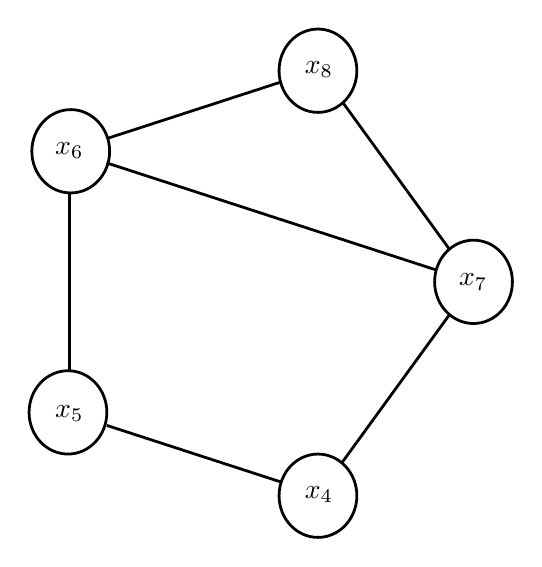
\begin{tikzpicture}[>=latex',line join=bevel,]
\pgfsetlinewidth{1bp}
\pgfsetcolor{black}
 \draw [solid] (15.5bp,59.46bp) .. controls (15.5bp,77.211bp) and (15.5bp,106.82bp)  .. (15.5bp,124.52bp);
 \draw [solid] (29.148bp,143.62bp) .. controls (46.136bp,149.14bp) and (74.968bp,158.5bp)  .. (91.878bp,164bp);
 \draw [solid] (152.46bp,103.55bp) .. controls (142.02bp,117.92bp) and (124.35bp,142.24bp)  .. (113.87bp,156.66bp);
 \draw [solid] (28.918bp,134.82bp) .. controls (56.617bp,125.82bp) and (119.84bp,105.28bp)  .. (147.51bp,96.289bp);
 \draw [solid] (113.79bp,27.11bp) .. controls (124.23bp,41.477bp) and (141.91bp,65.803bp)  .. (152.38bp,80.221bp);
 \draw [solid] (91.712bp,19.934bp) .. controls (74.724bp,25.454bp) and (45.892bp,34.822bp)  .. (28.982bp,40.317bp);
\begin{scope}
\definecolor{strokecol}{rgb}{0.0,0.0,0.0};
\pgfsetstrokecolor{strokecol}
\draw (105bp,168bp) ellipse (14bp and 15bp);
\draw (105.36bp,168.38bp) node {$x_8$};
\end{scope}
\begin{scope}
\definecolor{strokecol}{rgb}{0.0,0.0,0.0};
\pgfsetstrokecolor{strokecol}
\draw (16bp,139bp) ellipse (14bp and 15bp);
\draw (15.5bp,139.18bp) node {$x_6$};
\end{scope}
\begin{scope}
\definecolor{strokecol}{rgb}{0.0,0.0,0.0};
\pgfsetstrokecolor{strokecol}
\draw (161bp,92bp) ellipse (14bp and 15bp);
\draw (160.9bp,91.939bp) node {$x_7$};
\end{scope}
\begin{scope}
\definecolor{strokecol}{rgb}{0.0,0.0,0.0};
\pgfsetstrokecolor{strokecol}
\draw (105bp,15bp) ellipse (14bp and 15bp);
\draw (105.36bp,15.5bp) node {$x_4$};
\end{scope}
\begin{scope}
\definecolor{strokecol}{rgb}{0.0,0.0,0.0};
\pgfsetstrokecolor{strokecol}
\draw (15bp,45bp) ellipse (14bp and 15bp);
\draw (15.5bp,44.697bp) node {$x_5$};
\end{scope}
\end{tikzpicture}
%
%EndExpansion

\item Make $G_{NP}^{E}(\varphi _{1}^{E})$ chordal, using elimination
ordering $(x_{4,}x_{5,}x_{6,}x_{7,}x_{8})$:

%TCIMACRO{%
%\TeXButton{Chordal nonpolar equality graph }{\begin{tikzpicture}[>=latex',line join=bevel,]
%\pgfsetlinewidth{1bp}
%\pgfsetcolor{black}
% \draw [solid] (15.5bp,59.46bp) .. controls (15.5bp,77.211bp) and (15.5bp,106.82bp)  .. (15.5bp,124.52bp);
% \draw [solid] (29.148bp,143.62bp) .. controls (46.136bp,149.14bp) and (74.968bp,158.5bp)  .. (91.878bp,164bp);
% \draw [solid] (28.918bp,49.057bp) .. controls (56.617bp,58.057bp) and (119.84bp,78.599bp)  .. (147.51bp,87.59bp);
% \draw [solid] (152.46bp,103.55bp) .. controls (142.02bp,117.92bp) and (124.35bp,142.24bp)  .. (113.87bp,156.66bp);
% \draw [solid] (28.918bp,134.82bp) .. controls (56.617bp,125.82bp) and (119.84bp,105.28bp)  .. (147.51bp,96.289bp);
% \draw [solid] (113.79bp,27.11bp) .. controls (124.23bp,41.477bp) and (141.91bp,65.803bp)  .. (152.38bp,80.221bp);
% \draw [solid] (91.712bp,19.934bp) .. controls (74.724bp,25.454bp) and (45.892bp,34.822bp)  .. (28.982bp,40.317bp);
%\begin{scope}
%\definecolor{strokecol}{rgb}{0.0,0.0,0.0};
%\pgfsetstrokecolor{strokecol}
%\draw (105bp,168bp) ellipse (14bp and 15bp);
%\draw (105.36bp,168.38bp) node {$x_8$};
%\end{scope}
%\begin{scope}
%\definecolor{strokecol}{rgb}{0.0,0.0,0.0};
%\pgfsetstrokecolor{strokecol}
%\draw (16bp,139bp) ellipse (14bp and 15bp);
%\draw (15.5bp,139.18bp) node {$x_6$};
%\end{scope}
%\begin{scope}
%\definecolor{strokecol}{rgb}{0.0,0.0,0.0};
%\pgfsetstrokecolor{strokecol}
%\draw (161bp,92bp) ellipse (14bp and 15bp);
%\draw (160.9bp,91.939bp) node {$x_7$};
%\end{scope}
%\begin{scope}
%\definecolor{strokecol}{rgb}{0.0,0.0,0.0};
%\pgfsetstrokecolor{strokecol}
%\draw (105bp,15bp) ellipse (14bp and 15bp);
%\draw (105.36bp,15.5bp) node {$x_4$};
%\end{scope}
%\begin{scope}
%\definecolor{strokecol}{rgb}{0.0,0.0,0.0};
%\pgfsetstrokecolor{strokecol}
%\draw (15bp,45bp) ellipse (14bp and 15bp);
%\draw (15.5bp,44.697bp) node {$x_5$};
%\end{scope}
%\end{tikzpicture}
%}}%
%BeginExpansion
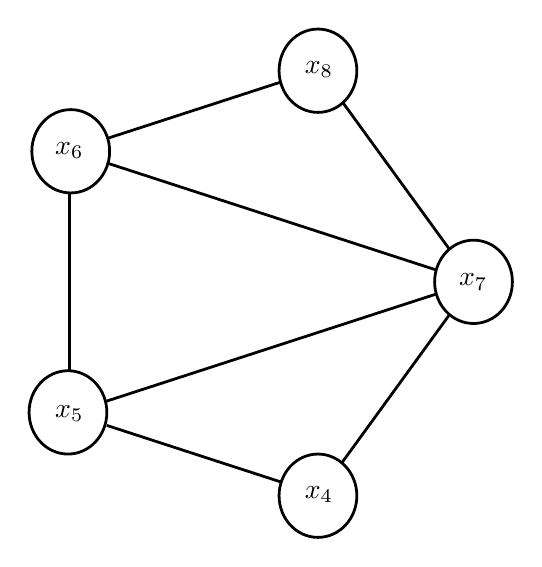
\begin{tikzpicture}[>=latex',line join=bevel,]
\pgfsetlinewidth{1bp}
\pgfsetcolor{black}
 \draw [solid] (15.5bp,59.46bp) .. controls (15.5bp,77.211bp) and (15.5bp,106.82bp)  .. (15.5bp,124.52bp);
 \draw [solid] (29.148bp,143.62bp) .. controls (46.136bp,149.14bp) and (74.968bp,158.5bp)  .. (91.878bp,164bp);
 \draw [solid] (28.918bp,49.057bp) .. controls (56.617bp,58.057bp) and (119.84bp,78.599bp)  .. (147.51bp,87.59bp);
 \draw [solid] (152.46bp,103.55bp) .. controls (142.02bp,117.92bp) and (124.35bp,142.24bp)  .. (113.87bp,156.66bp);
 \draw [solid] (28.918bp,134.82bp) .. controls (56.617bp,125.82bp) and (119.84bp,105.28bp)  .. (147.51bp,96.289bp);
 \draw [solid] (113.79bp,27.11bp) .. controls (124.23bp,41.477bp) and (141.91bp,65.803bp)  .. (152.38bp,80.221bp);
 \draw [solid] (91.712bp,19.934bp) .. controls (74.724bp,25.454bp) and (45.892bp,34.822bp)  .. (28.982bp,40.317bp);
\begin{scope}
\definecolor{strokecol}{rgb}{0.0,0.0,0.0};
\pgfsetstrokecolor{strokecol}
\draw (105bp,168bp) ellipse (14bp and 15bp);
\draw (105.36bp,168.38bp) node {$x_8$};
\end{scope}
\begin{scope}
\definecolor{strokecol}{rgb}{0.0,0.0,0.0};
\pgfsetstrokecolor{strokecol}
\draw (16bp,139bp) ellipse (14bp and 15bp);
\draw (15.5bp,139.18bp) node {$x_6$};
\end{scope}
\begin{scope}
\definecolor{strokecol}{rgb}{0.0,0.0,0.0};
\pgfsetstrokecolor{strokecol}
\draw (161bp,92bp) ellipse (14bp and 15bp);
\draw (160.9bp,91.939bp) node {$x_7$};
\end{scope}
\begin{scope}
\definecolor{strokecol}{rgb}{0.0,0.0,0.0};
\pgfsetstrokecolor{strokecol}
\draw (105bp,15bp) ellipse (14bp and 15bp);
\draw (105.36bp,15.5bp) node {$x_4$};
\end{scope}
\begin{scope}
\definecolor{strokecol}{rgb}{0.0,0.0,0.0};
\pgfsetstrokecolor{strokecol}
\draw (15bp,45bp) ellipse (14bp and 15bp);
\draw (15.5bp,44.697bp) node {$x_5$};
\end{scope}
\end{tikzpicture}
%
%EndExpansion

\item Generate the transitivity constraints in $B_{t}$ for every triangle in
the chordal graph $G_{NP}^{E}(\varphi _{1}^{E})$:

\begin{enumerate}
\item $B_{t}=$ \textsc{True}

\item for each triangle $(e_{i,j},e_{j,k},e_{i,k})$ in $G_{NP}^{E}(\varphi
_{1}^{E})$:%
\begin{eqnarray*}
B_{t}=((e_{4,5}\AND e_{5,7}\IMPL e_{4,7})\AND && \\
(e_{4,5}\AND e_{4,7}\IMPL e_{5,7})\AND && \\
(e_{4,7}\AND e_{5,7}\IMPL e_{4,5})\AND && \\
(e_{5,6}\AND e_{6,7}\IMPL e_{5,7})\AND && \\
(e_{5,6}\AND e_{5,7}\IMPL e_{6,7})\AND && \\
(e_{5,7}\AND e_{6,7}\IMPL e_{5,6})\AND && \\
(e_{6,7}\AND e_{7,8}\IMPL e_{6,8})\AND && \\
(e_{6,7}\AND e_{6,8}\IMPL e_{7,8})\AND && \\
(e_{6,8}\AND e_{7,8}\IMPL e_{6,7})) &&
\end{eqnarray*}

Hence, $\varphi ^{E}$ is satisfiable, iff $\varphi ^{P}=e(\varphi _{1}^{E})%
\AND B_{t}$ is satisfiable.
\end{enumerate}
\end{enumerate}


  }


%%%%%%%%%%%%%%%%%%%%%%%%%%%%%%%%%%%%%%%%%%%%%%%%%%%%%%%%%%%%%%%%%%%%%%%%%%%%%%

\newpage
\Aufgabe[Ackermann's Reduction \hfill \bf (1 point)]
Apply Ackermann's reduction on the following EUF-formula $\varphi$ to obtain
an EU formula:
\begin{displaymath}
  f\left(f\left(g\left(a\right),b\right),a\right) = f(g(a),b) \rightarrow \big[ f(x,y) = g(f(g(a),b)) \land
  g(f(a,y))=d \big]
\end{displaymath}


\solution{
}


\end{document}
